\beginsong{Tra boschi e prati}

\begin{tikzpicture}[remember picture, overlay]
    \node[opacity=0.15, inner sep=0pt, anchor=south east] 
    at (current page text area.south east) { % Centra l'immagine nella pagina
        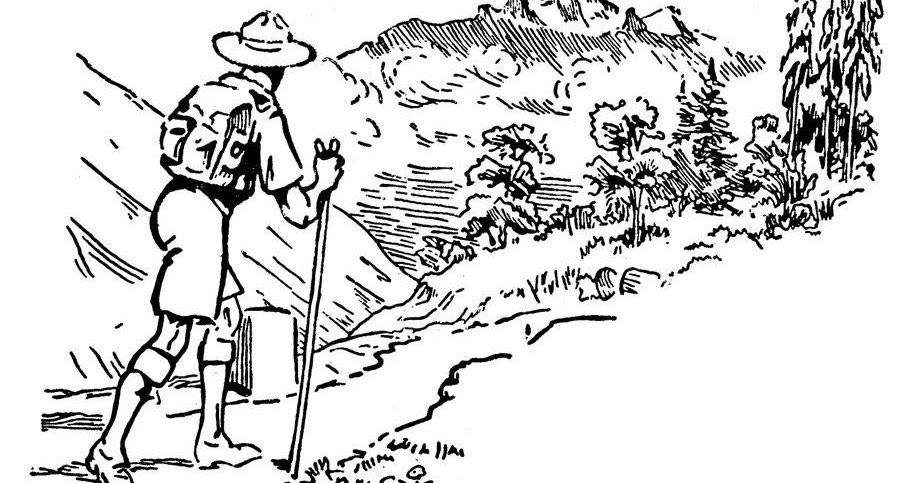
\includegraphics[width=\paperwidth]{img/cammino.png} 
    };
\end{tikzpicture}

\beginverse

\[LAm]Tra boschi prati \[DO]verdi e fiumi 
con l'\[SOL]acqua e con il \[LAm]sole
col vento oppure con l'\[DO]aria lieve 
nella \[SOL]calda estate o \[LAm]con la neve
\[FA]Quanti passi \[DO]fatti assieme al\[SOL]legria di una fa\[LAm]tica
\[FA]ancor più me\[DO]ravigliosa per\[SOL]ché \dots
fatta con \[LAm]te \[SOL] \rep{2}

\endverse

\chordsoff

\beginverse

Un sorso d'acqua fresca e poi 
l'orizzonte di nuovo davanti a noi
e senza più limiti ed ore 
ci fermeremo col morir del sole
Per poi star davanti al fuoco 
in una notte con la luna
a pregar le stelle e il vento di \dots
portarci la fortuna

\endverse

\beginverse

Lo zaino è fatto tutto è pronto 
un nuovo giorno è sorto già
e con il ritmo dei nostri passi 
il nostro tempo misurerem
poi di nuovo sul sentiero 
solitario e silenzioso
testimone delle fatiche di chi \dots
in alto vuole andar 

\endverse

\endsong
